% !TeX root = ../thuthesis-example.tex

\chapter{行人检测与高斯概率分布建模}

\section{数据集扩充和预处理}

对于行人检测与高斯概率分布建模,首先需要选择合适的数据集,并对数据进行预处理。目前,比较适合多摄像头多目标位置估计的综合性能较好的数据集主要包括Duke MTMC(Multi-Target, Multi-Camera)数据集\cite{Ristani2016PerformanceMA}和上文提到的WildTrack数据集。其中,Duke MTMC数据集是2014年杜克大学校园拍摄的监控视频片段的数据集,用于视频跟踪系统、行人重识别和低分辨率面部识别的研发。这个数据集包含超过14小时的来自8个摄像头的同步监控视频,视频为1080p和60fps,超过200万帧,其中共有2000名学生步行上下学。但由于英国《金融时报》调查发现此数据集可能侵犯个人隐私,Duke MTMC数据集关闭了下载渠道。而WildTrack数据集则是一个记录了苏黎世联邦理工大学主楼外的学生的监控录像数据集。WildTrack使用七个具有重叠视野的高科技静态定位摄像头(三个GoPro Hero 4和四个GoPro Hero 3摄像头)获取,具有高精度的联合摄像机校准以及视图序列同步,并且摄像头视野有着较大部分的重叠。因此可以满足在多视角多目标位置估计问题中大规模多摄像头数据集深度学习训练的需要。

本文采用WildTrack数据集。此数据集提供了时长为35分钟的分辨率为$1920\times1080$、帧率为60fps的来自七个摄像头的同步视频,以及分辨率为$1920\times1080$、帧率为2fps并消除畸变后的400张视频帧(如图~\ref{WildTrack_Cam}所示),并且提供了400张视频帧的行人位置标注,最后,还提供了每个摄像头的相机参数。此数据集所关注的区域为$1200cm\times3600cm$广场,而在标注时,将广场分割为$480\times1440$的网格,每个网格边长为2.5cm,从而得到691200个网格点。对每个网格点从上到下从左到右进行编号,可以得到网格编号,称为Position ID。若在此网格上建立直角坐标系,坐标以米为单位,原点在$(-3.0, -9.0)$处,从而,根据Position ID可以得到标注坐标为
\begin{equation*}
  \left\{
    \begin{aligned}
    X = & -3.0 + 0.025 \times \text{Position ID} \% 480 \\\
    Y = & -9.0 + 0.025 \times \text{Position ID} / 480
    \end{aligned}
  \right.
\end{equation*}


\begin{figure}
    \centering
    \subcaptionbox{\label{cam1}}
      {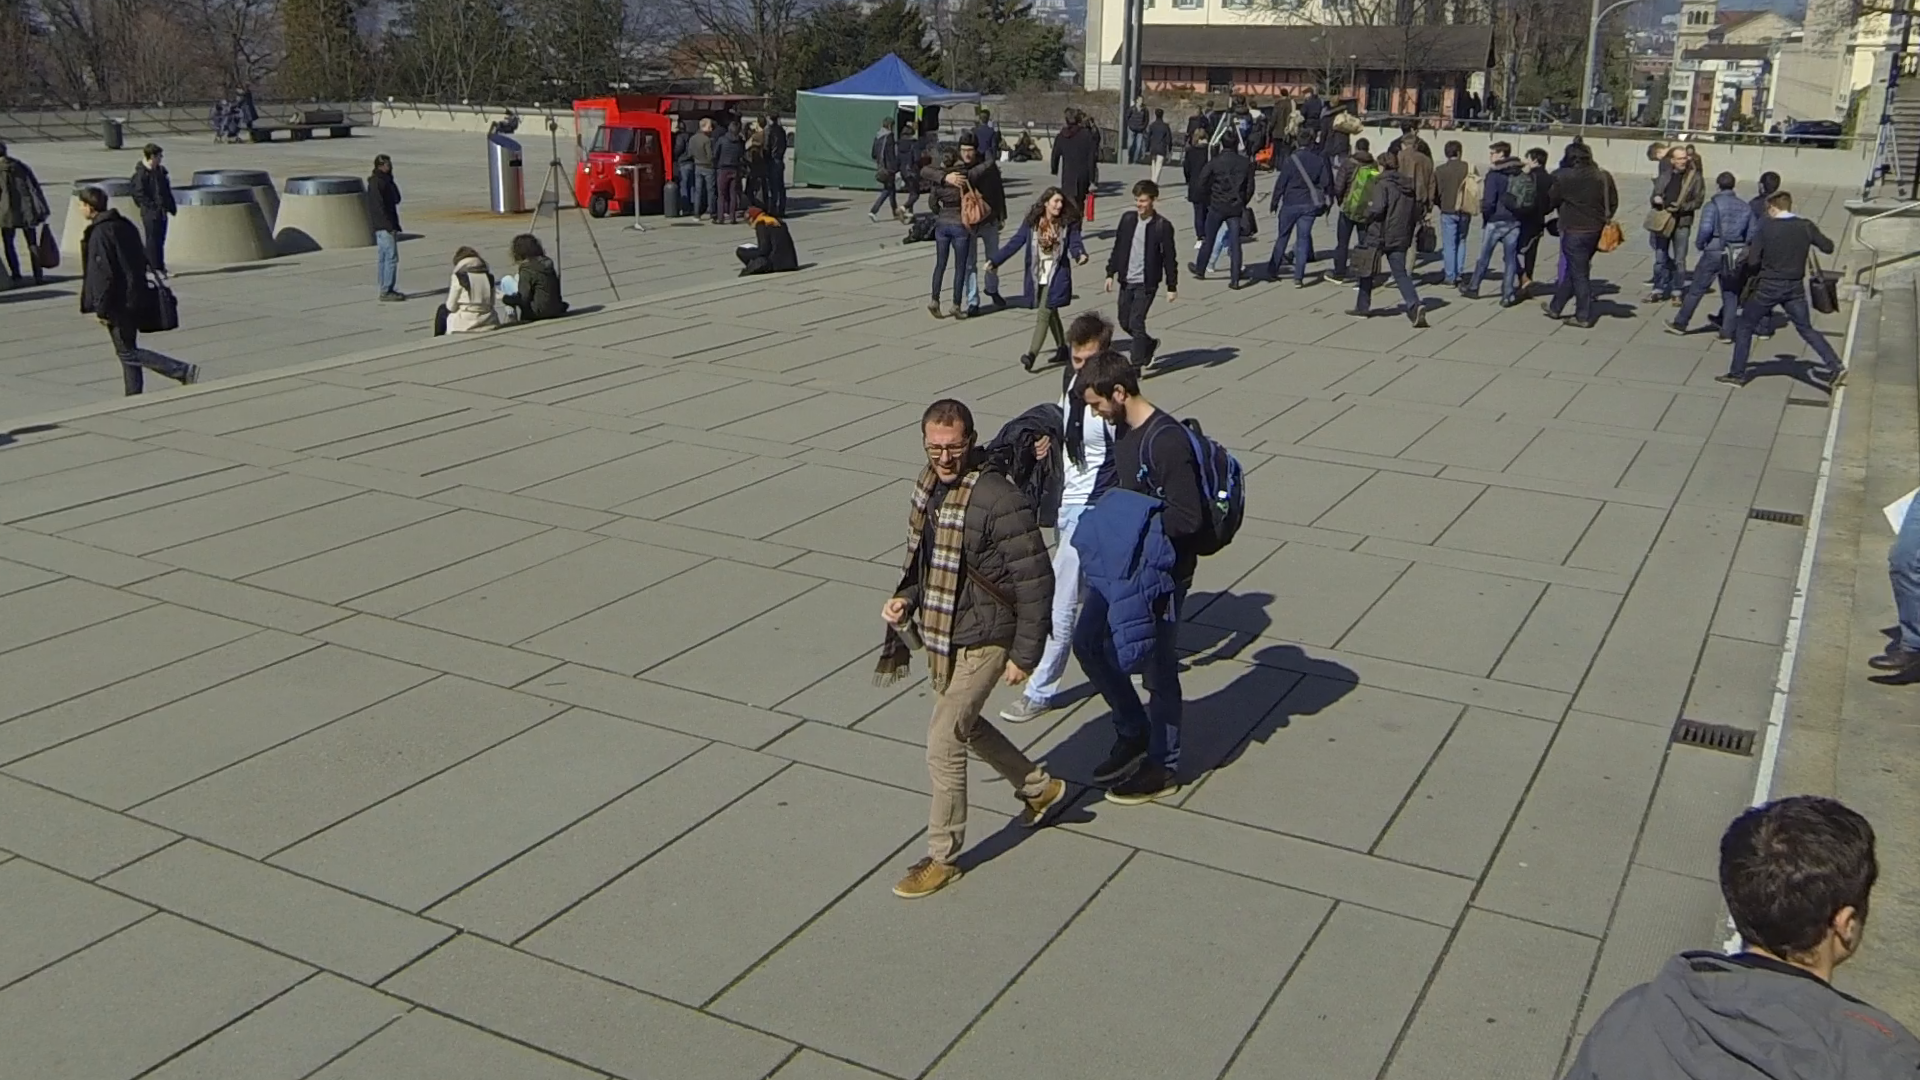
\includegraphics[width=0.3\linewidth]{cam1.png}}
    \subcaptionbox{\label{cam2}}
      {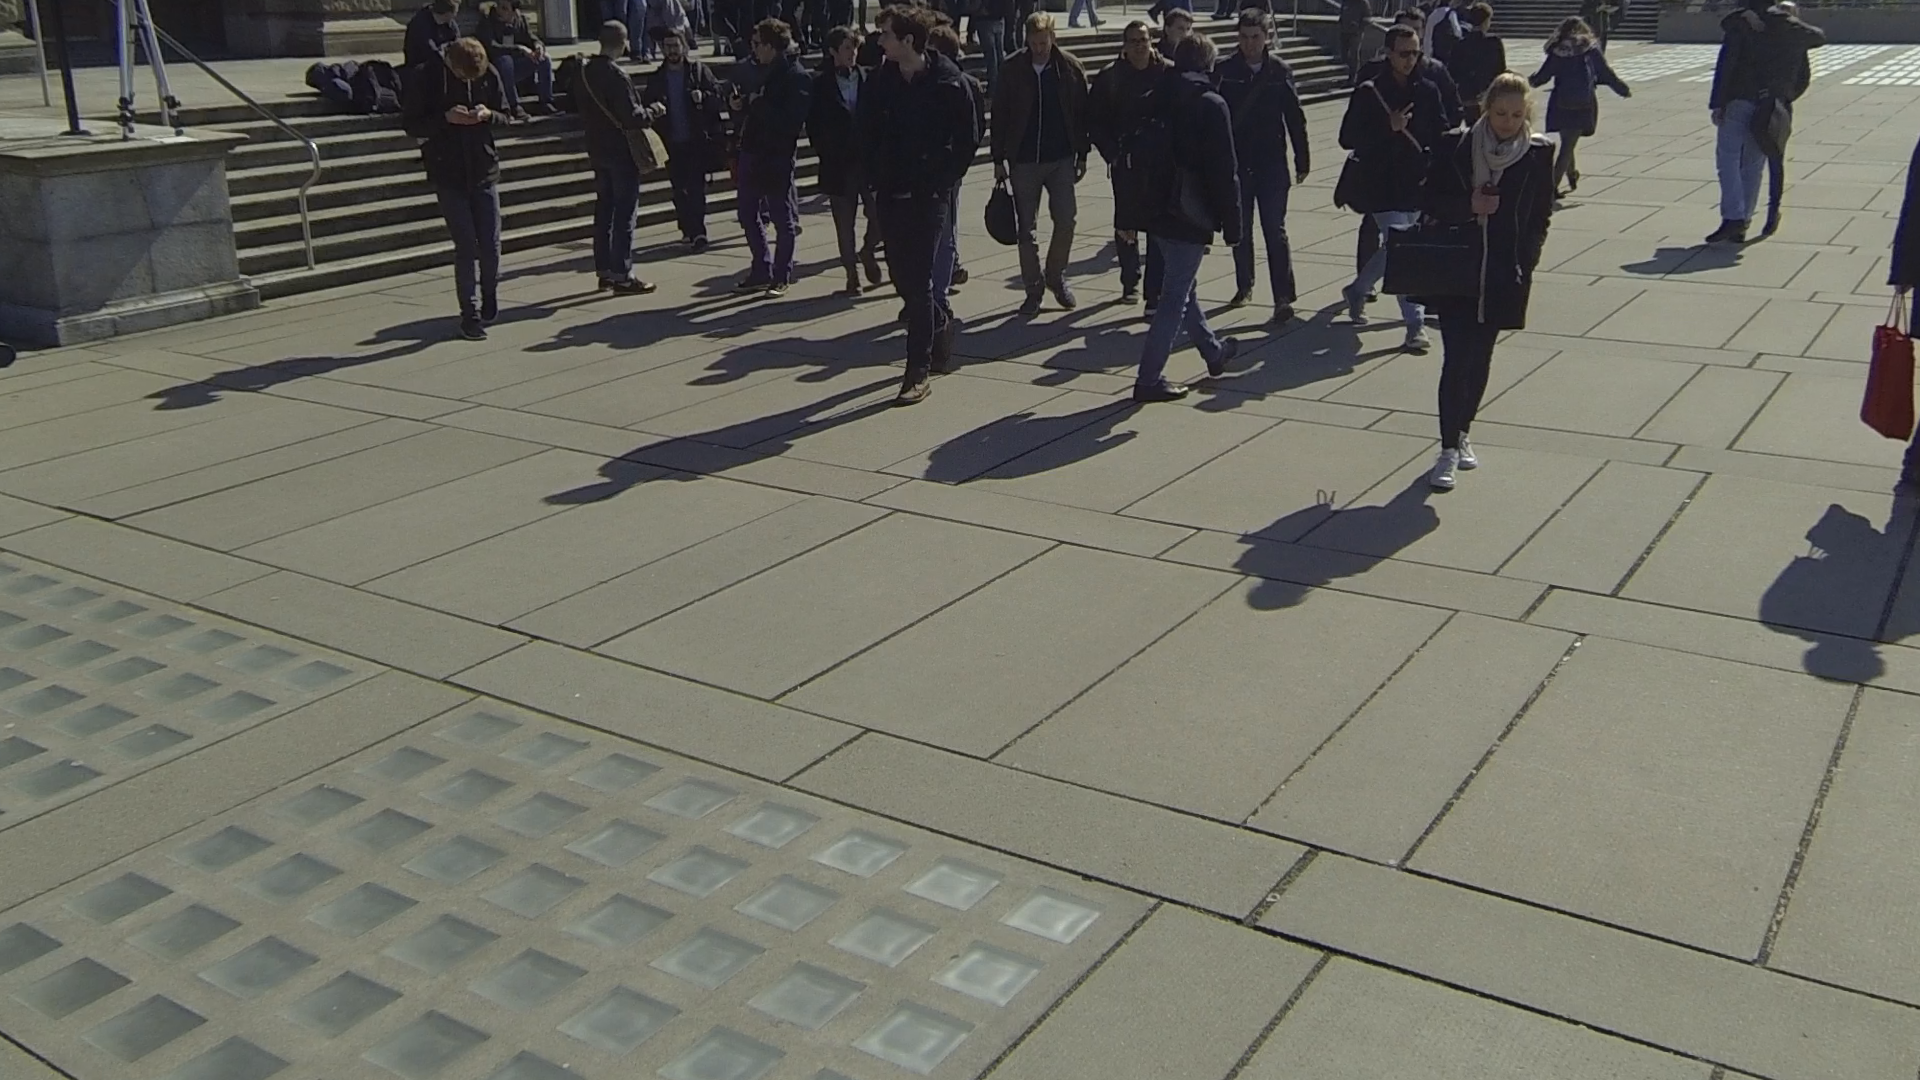
\includegraphics[width=0.3\linewidth]{cam2.png}}
    \subcaptionbox{\label{cam3}}
      {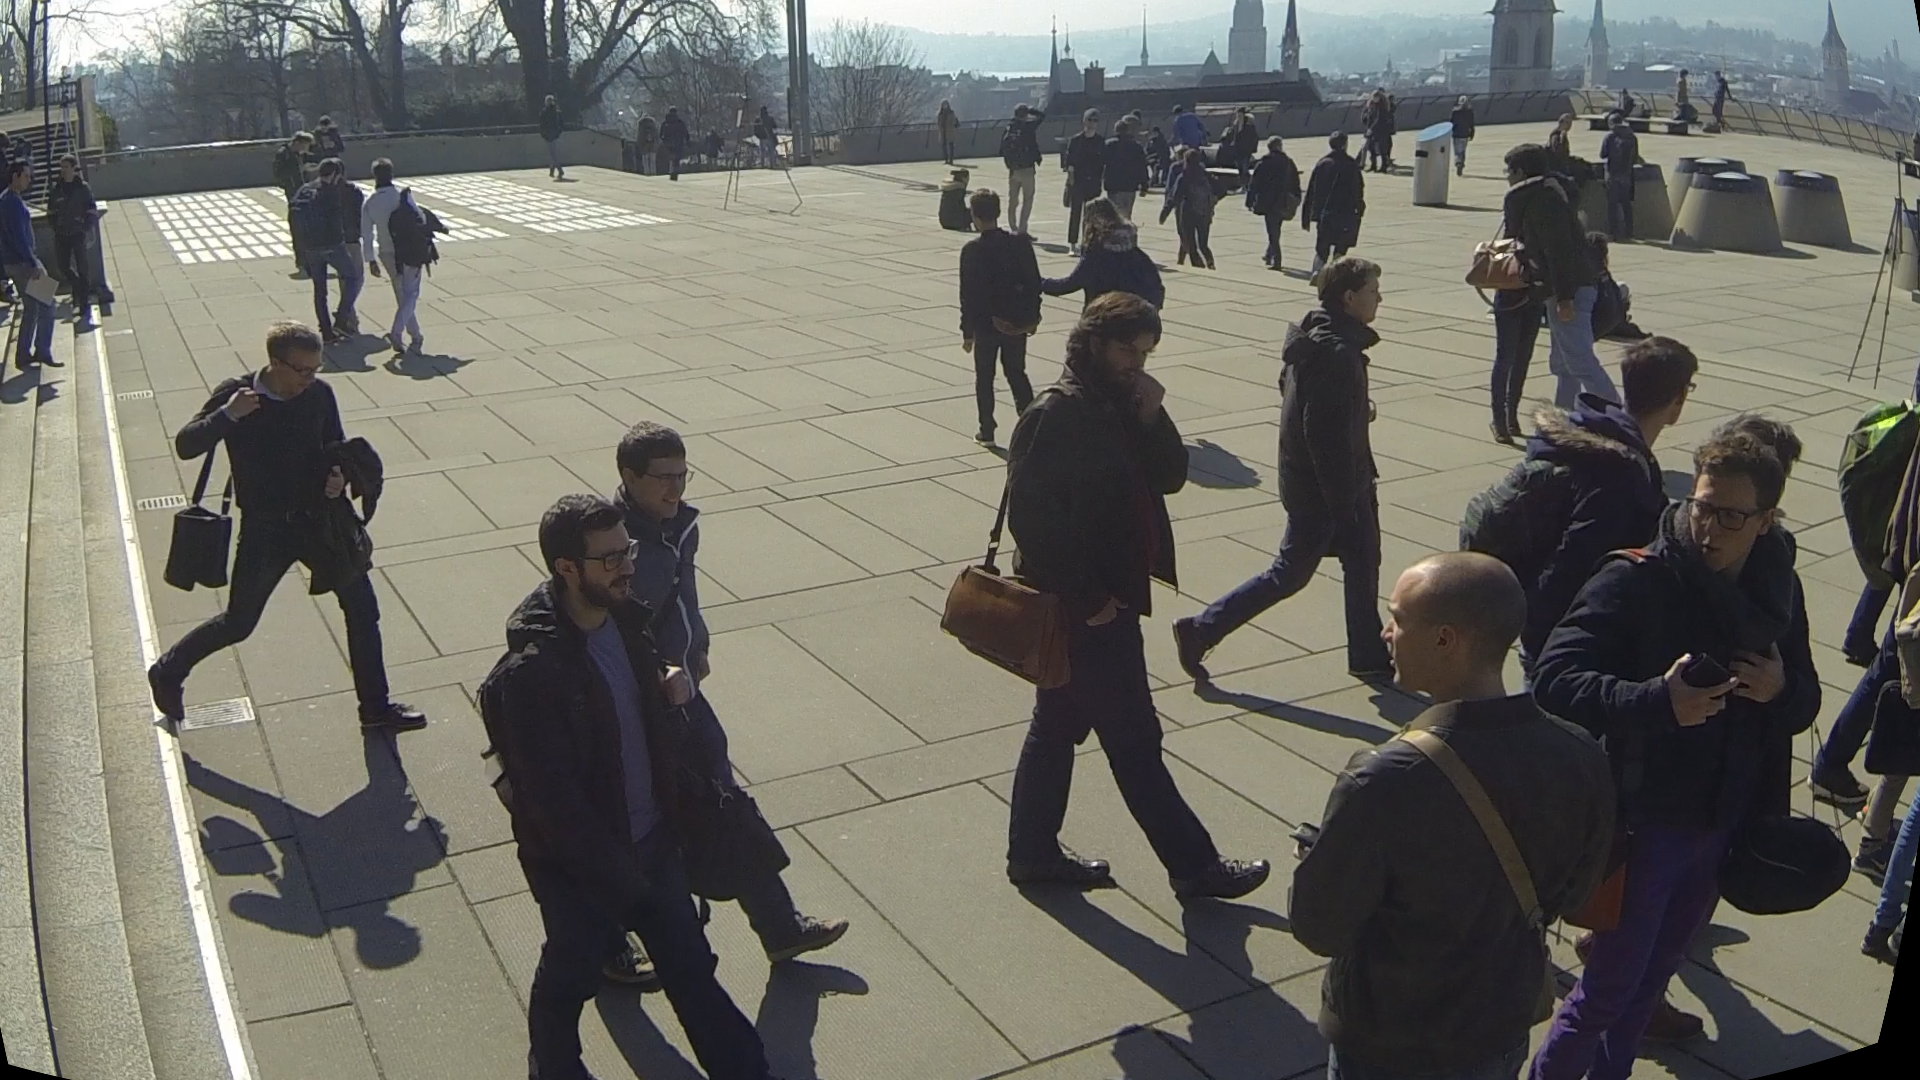
\includegraphics[width=0.3\linewidth]{cam3.png}}
    \quad
    \subcaptionbox{\label{cam4}}
      {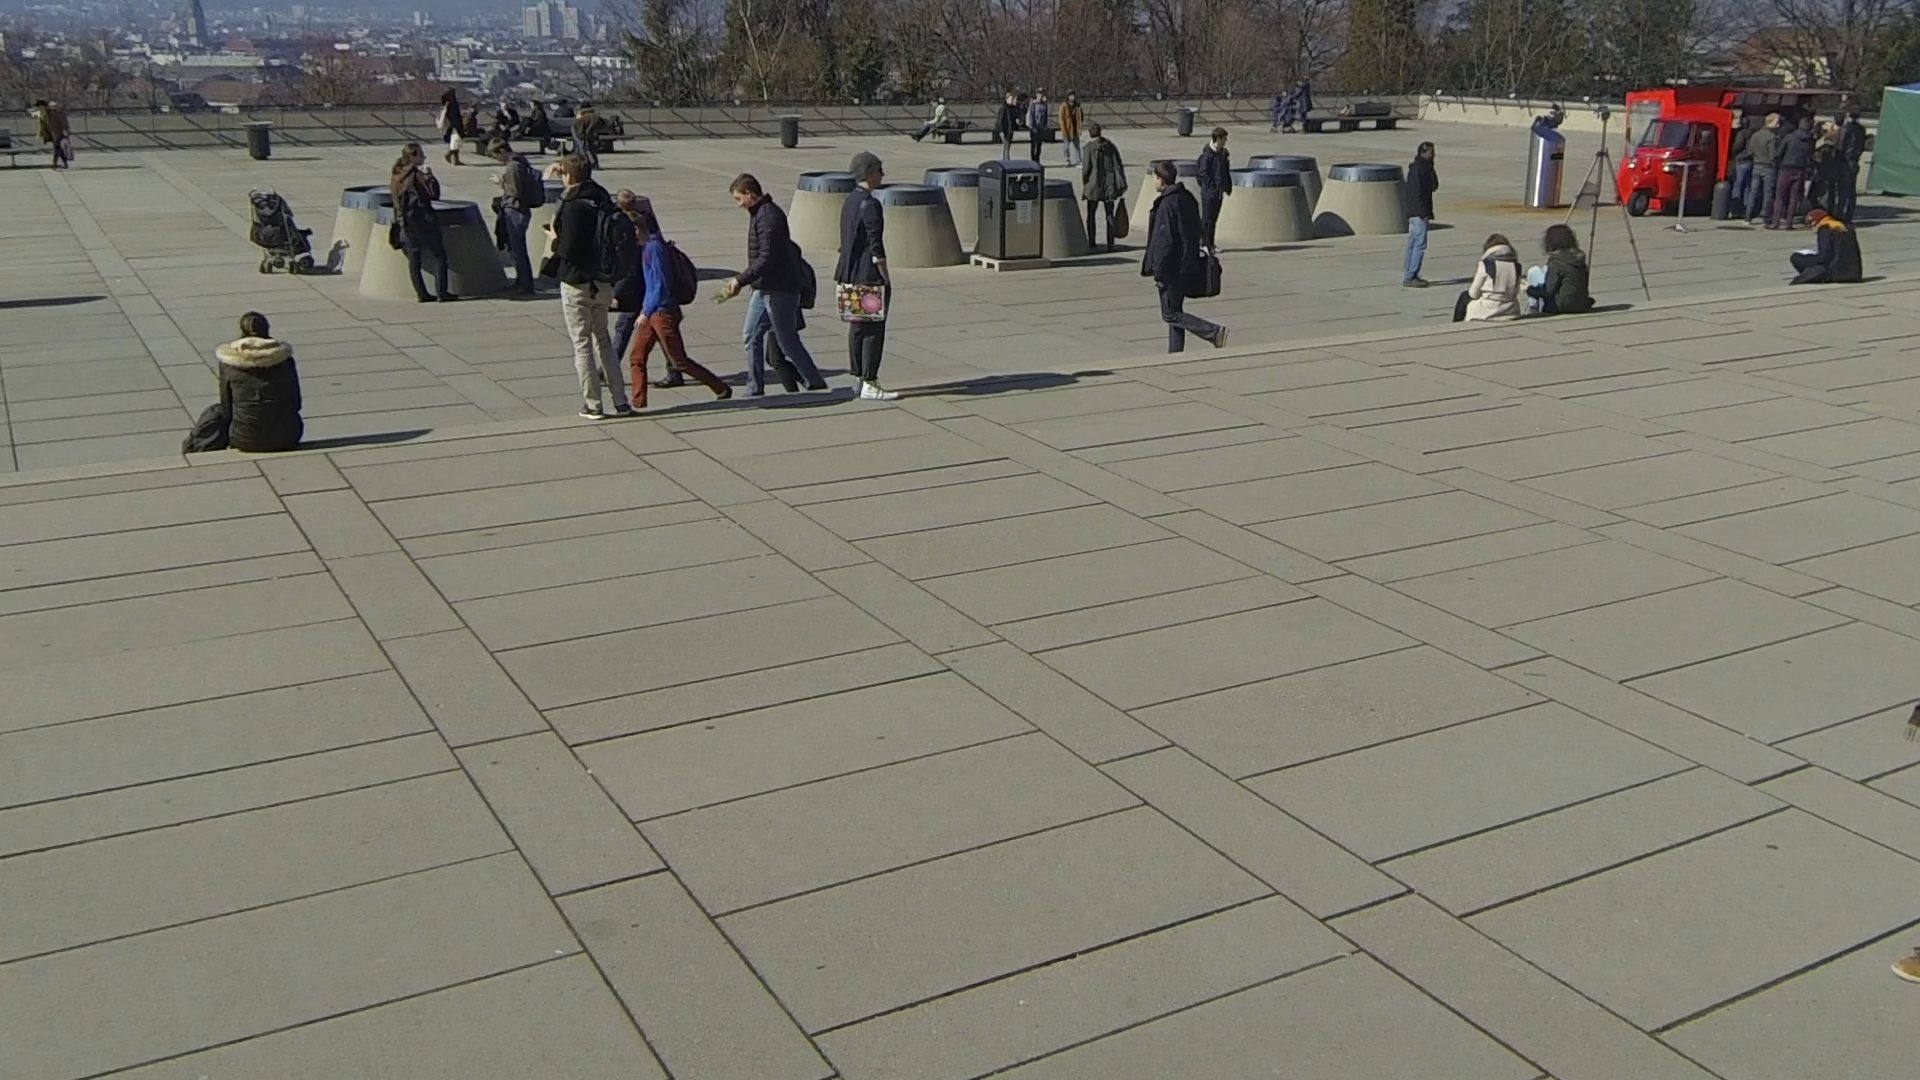
\includegraphics[width=0.3\linewidth]{cam4.png}}
    \subcaptionbox{\label{cam5}}
      {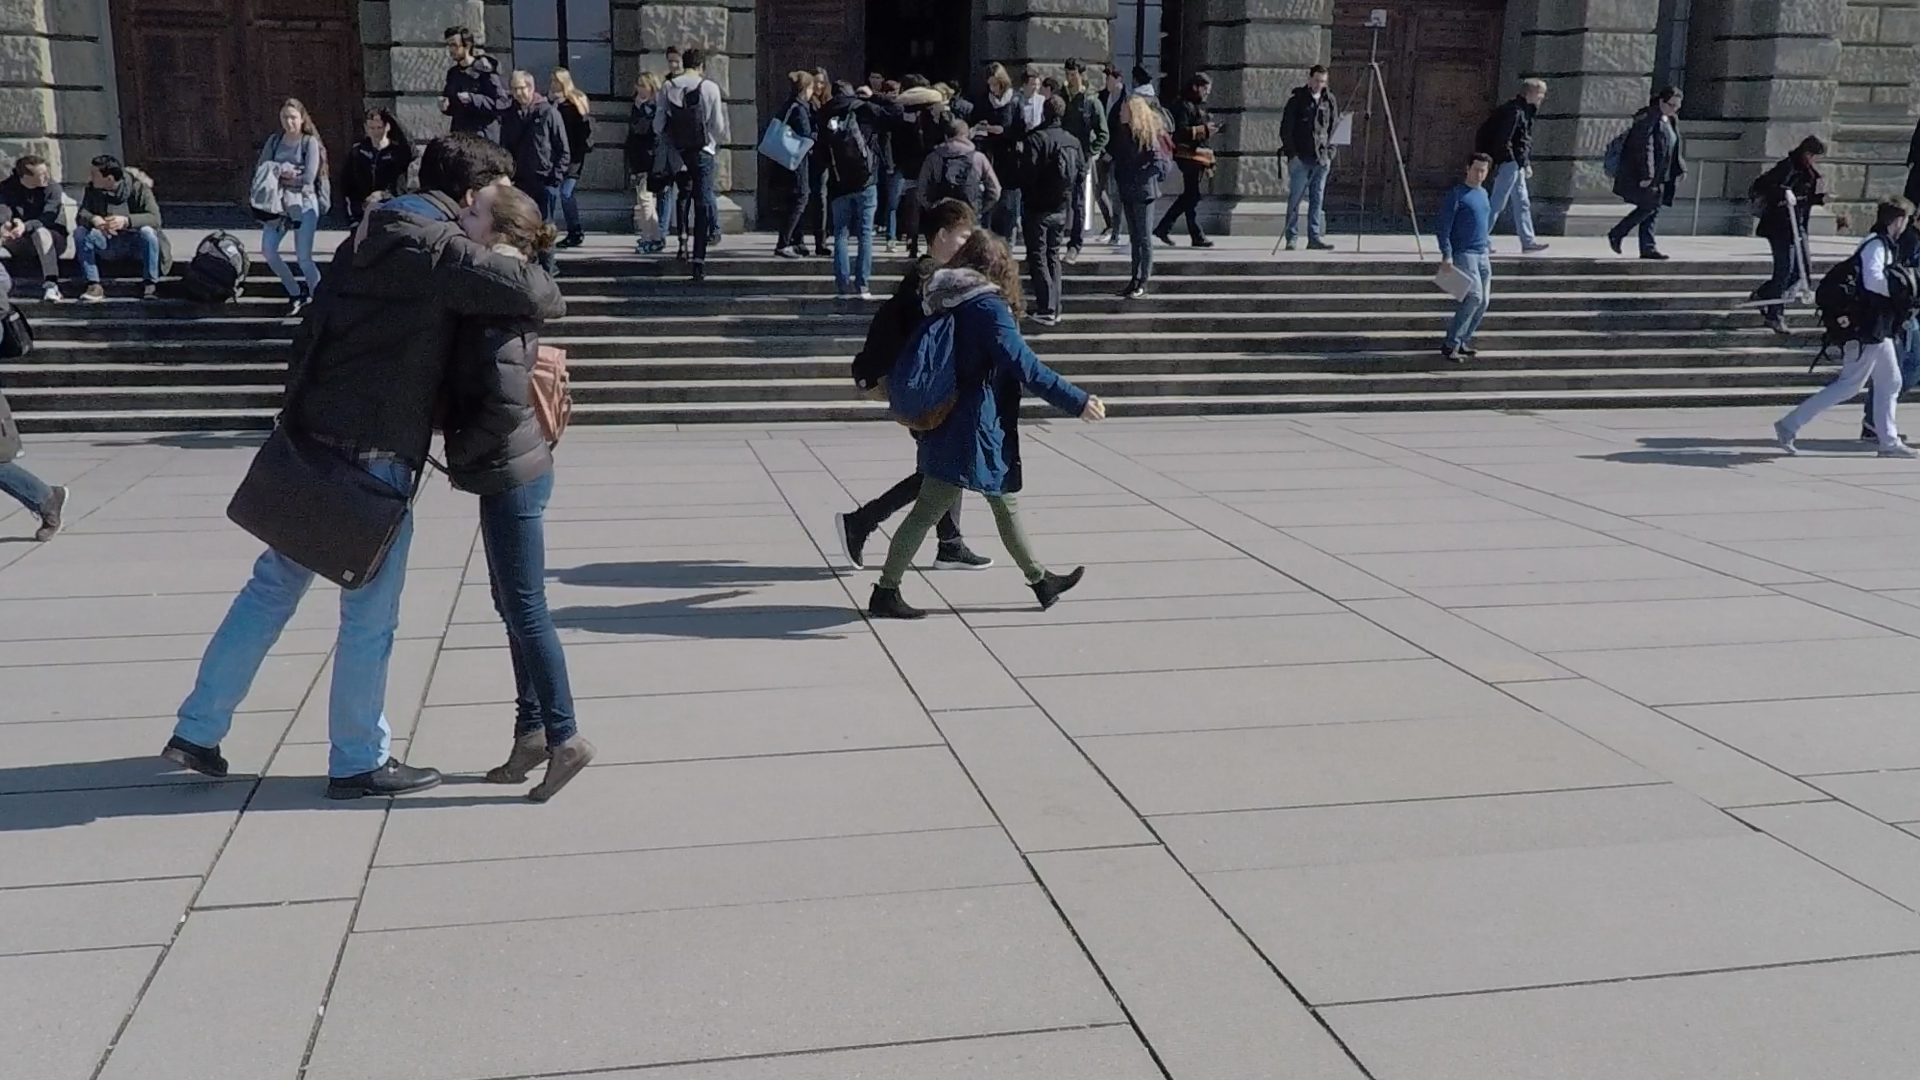
\includegraphics[width=0.3\linewidth]{cam5.png}}
    \subcaptionbox{\label{cam6}}
      {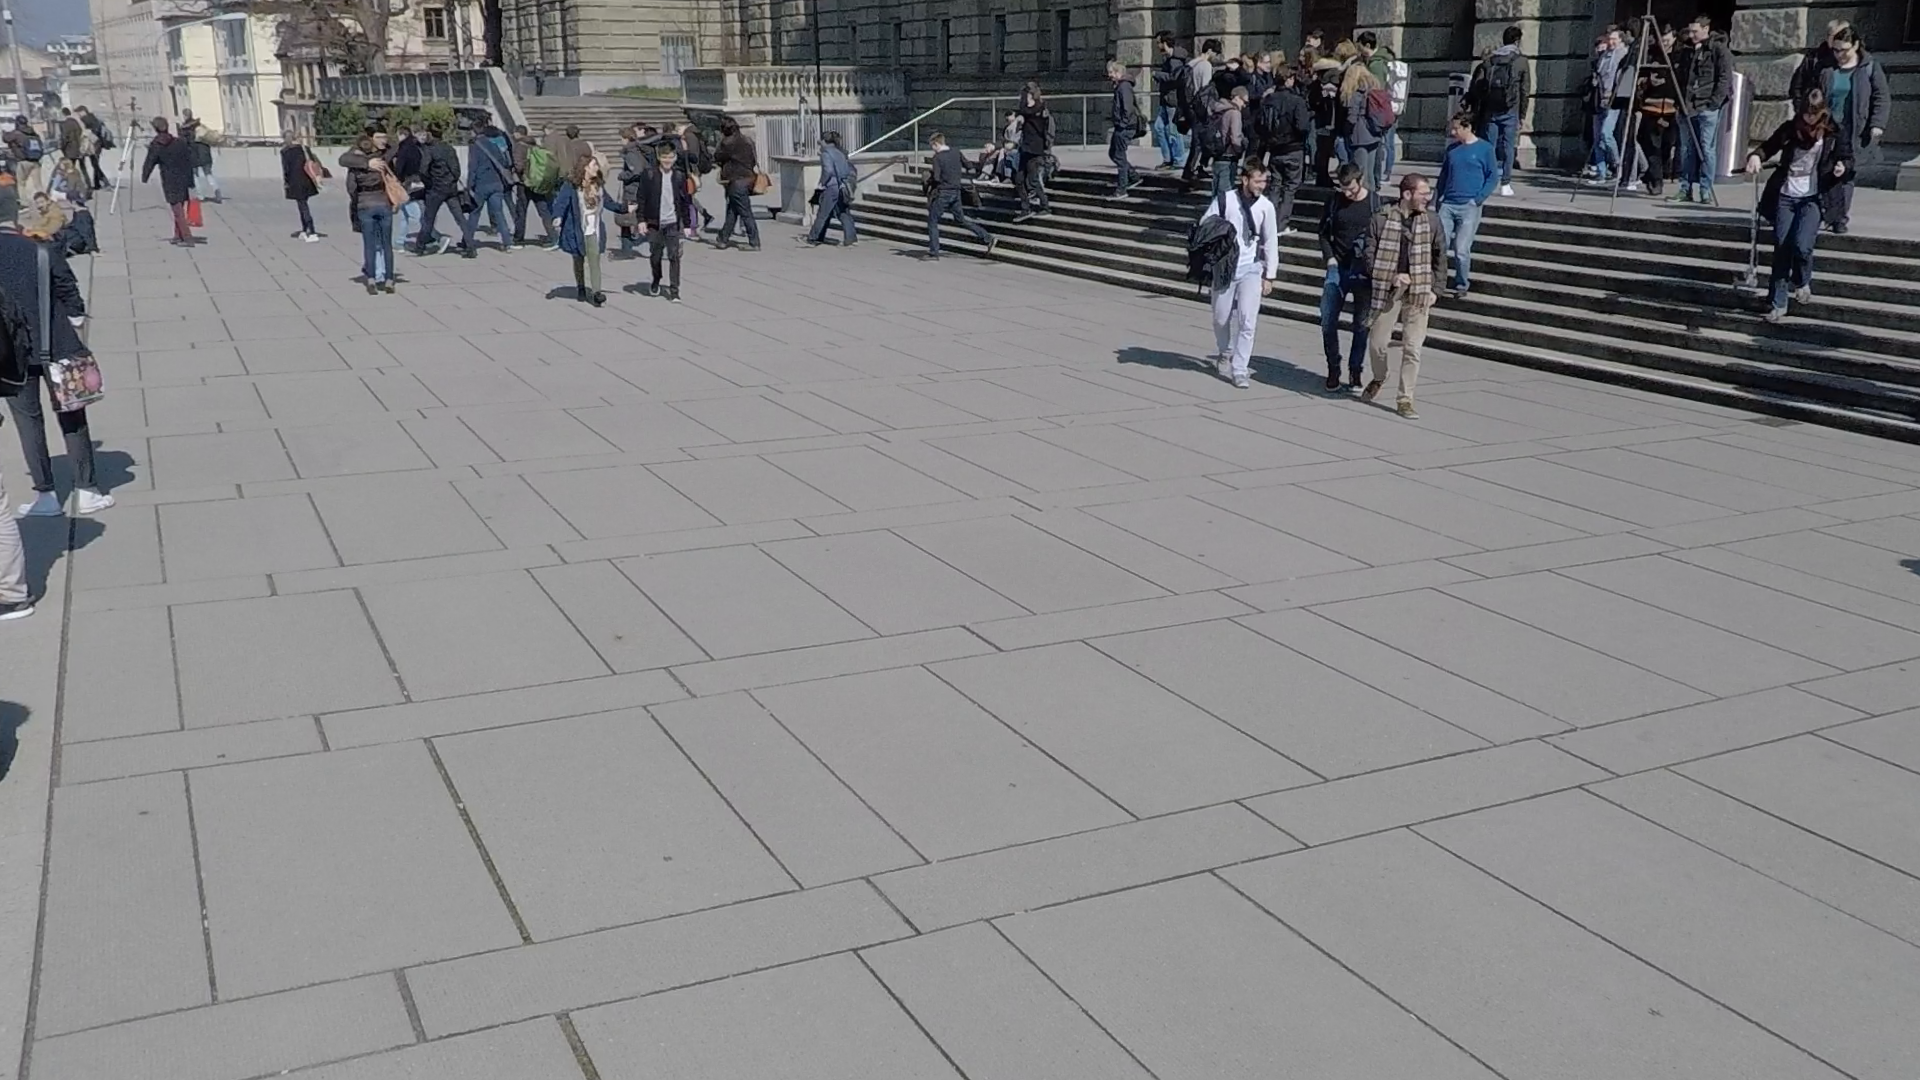
\includegraphics[width=0.3\linewidth]{cam6.png}}
    \subcaptionbox{\label{cam7}}
      {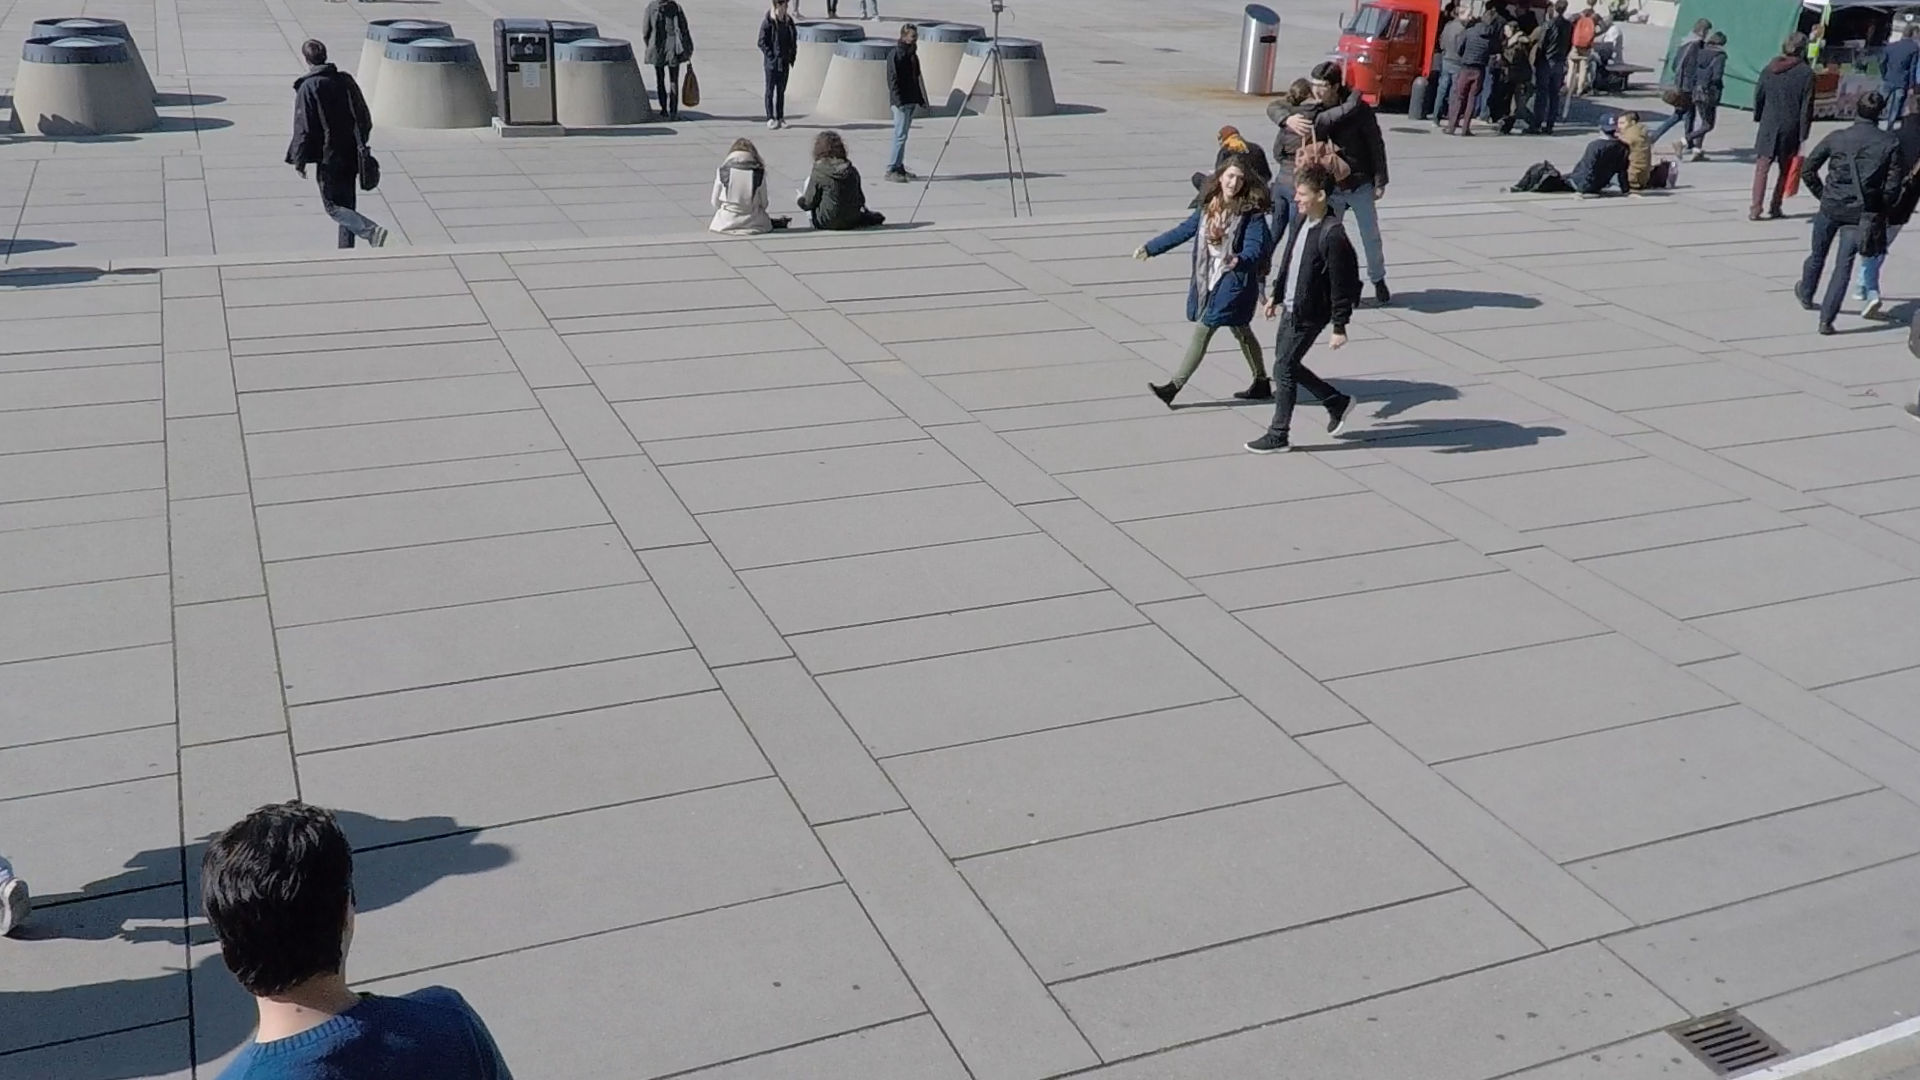
\includegraphics[width=0.3\linewidth]{cam7.png}}
    \caption{WildTrack数据集中来自七个摄像头的图片}
    \label{WildTrack_Cam}
\end{figure}

由于后续神经网络训练的需要,而官方提供的400张图片和标注总体数量太少,难以达到预期训练效果,因此需要使用WildTrack数据集提供的视频进行数据集的扩充。由于带标注的400张图片帧率为2fps,而视频序列的帧率则为60fps,因此,可以先从视频序列中找到与官方提供的图片集一致的帧,以此帧为起点,每30帧就会再次遇到官方图片集中的下一张图片。但是,由于从视频序列中提取的帧在WildTrack数据集中并不提供真值标注,因此可以通过对提供标注的400张图片集的标注进行插值,从而推断得到每两个图片之间提取到的视频帧的真值标注。此外,由于提供的图片集已经被去畸变处理过,而提取到的视频帧并未去畸变处理。故需要先对视频帧进行与图片集相同的去畸变处理,如图~\ref{undistortion}所示。

\begin{figure}
  \centering
  \subcaptionbox{\label{before}}
    {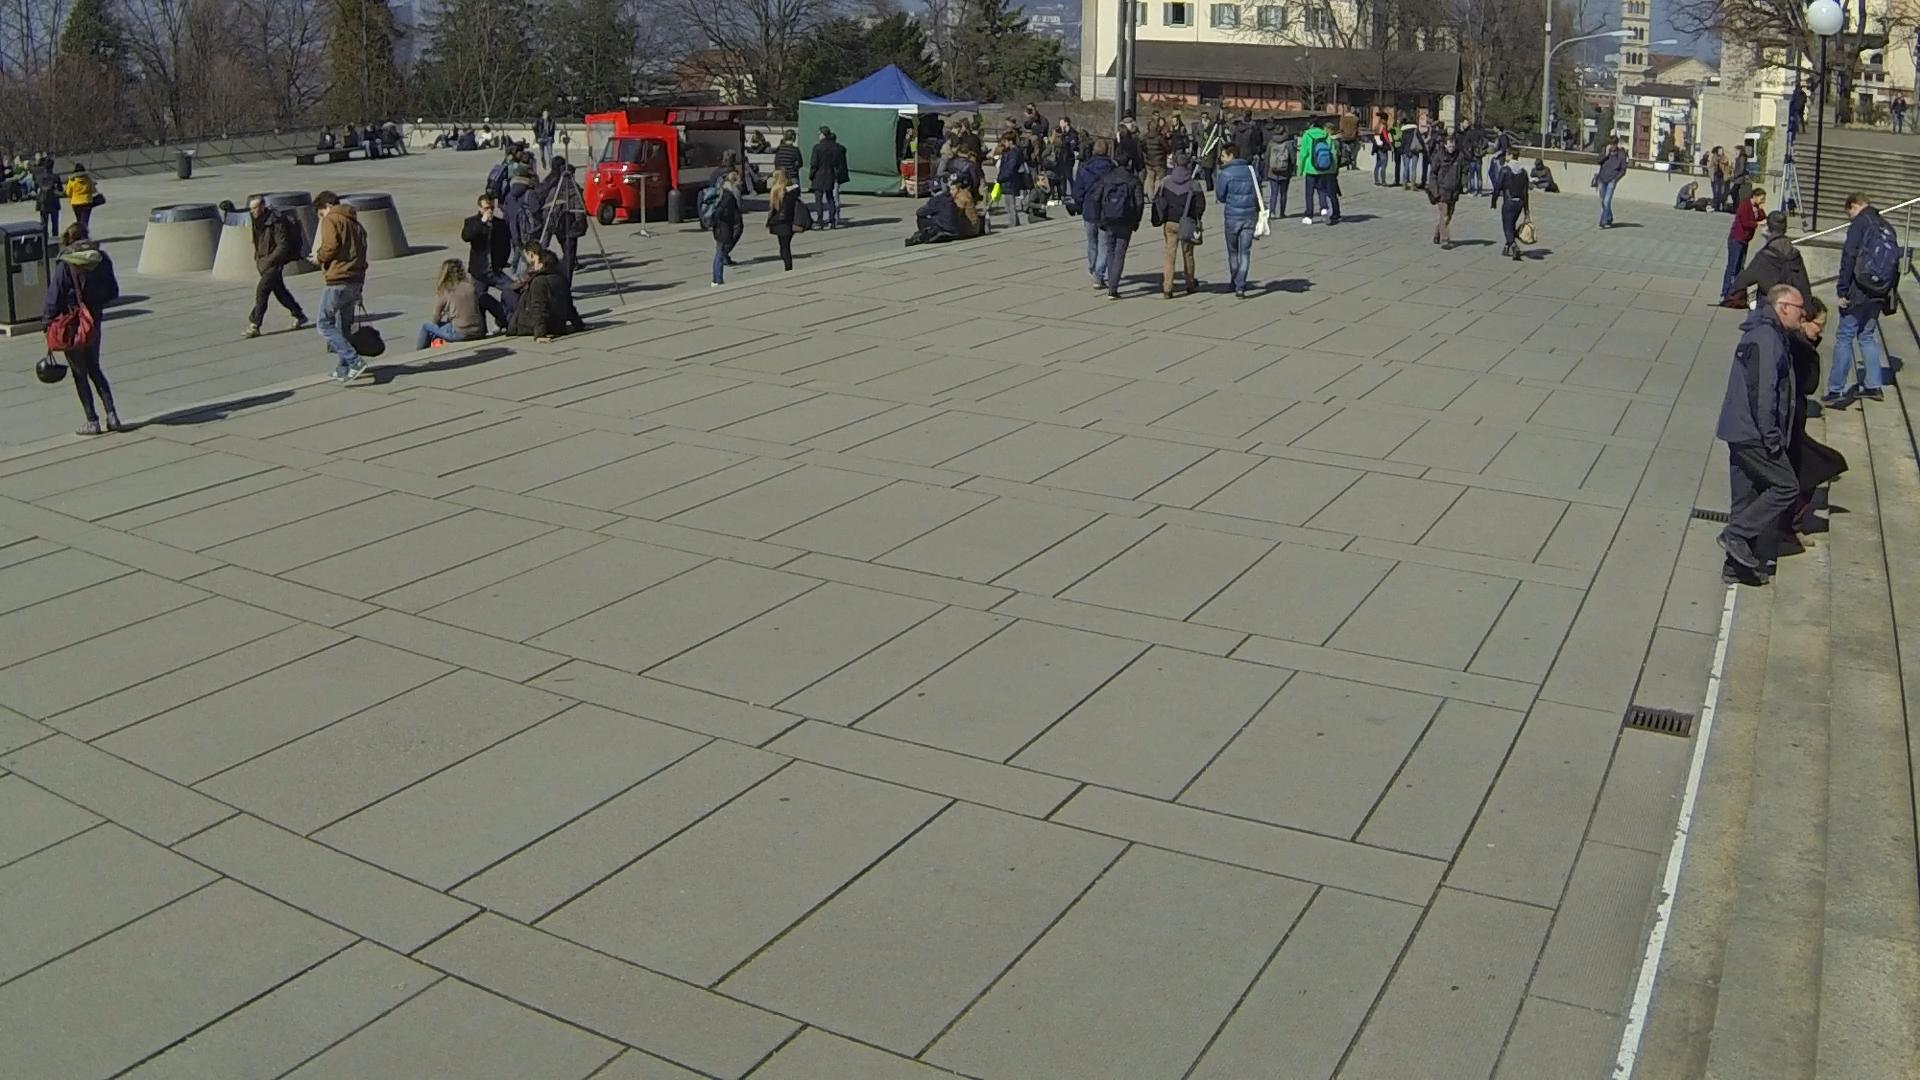
\includegraphics[width=0.4\linewidth]{before_undistort.jpg}}
  \subcaptionbox{\label{after}}
    {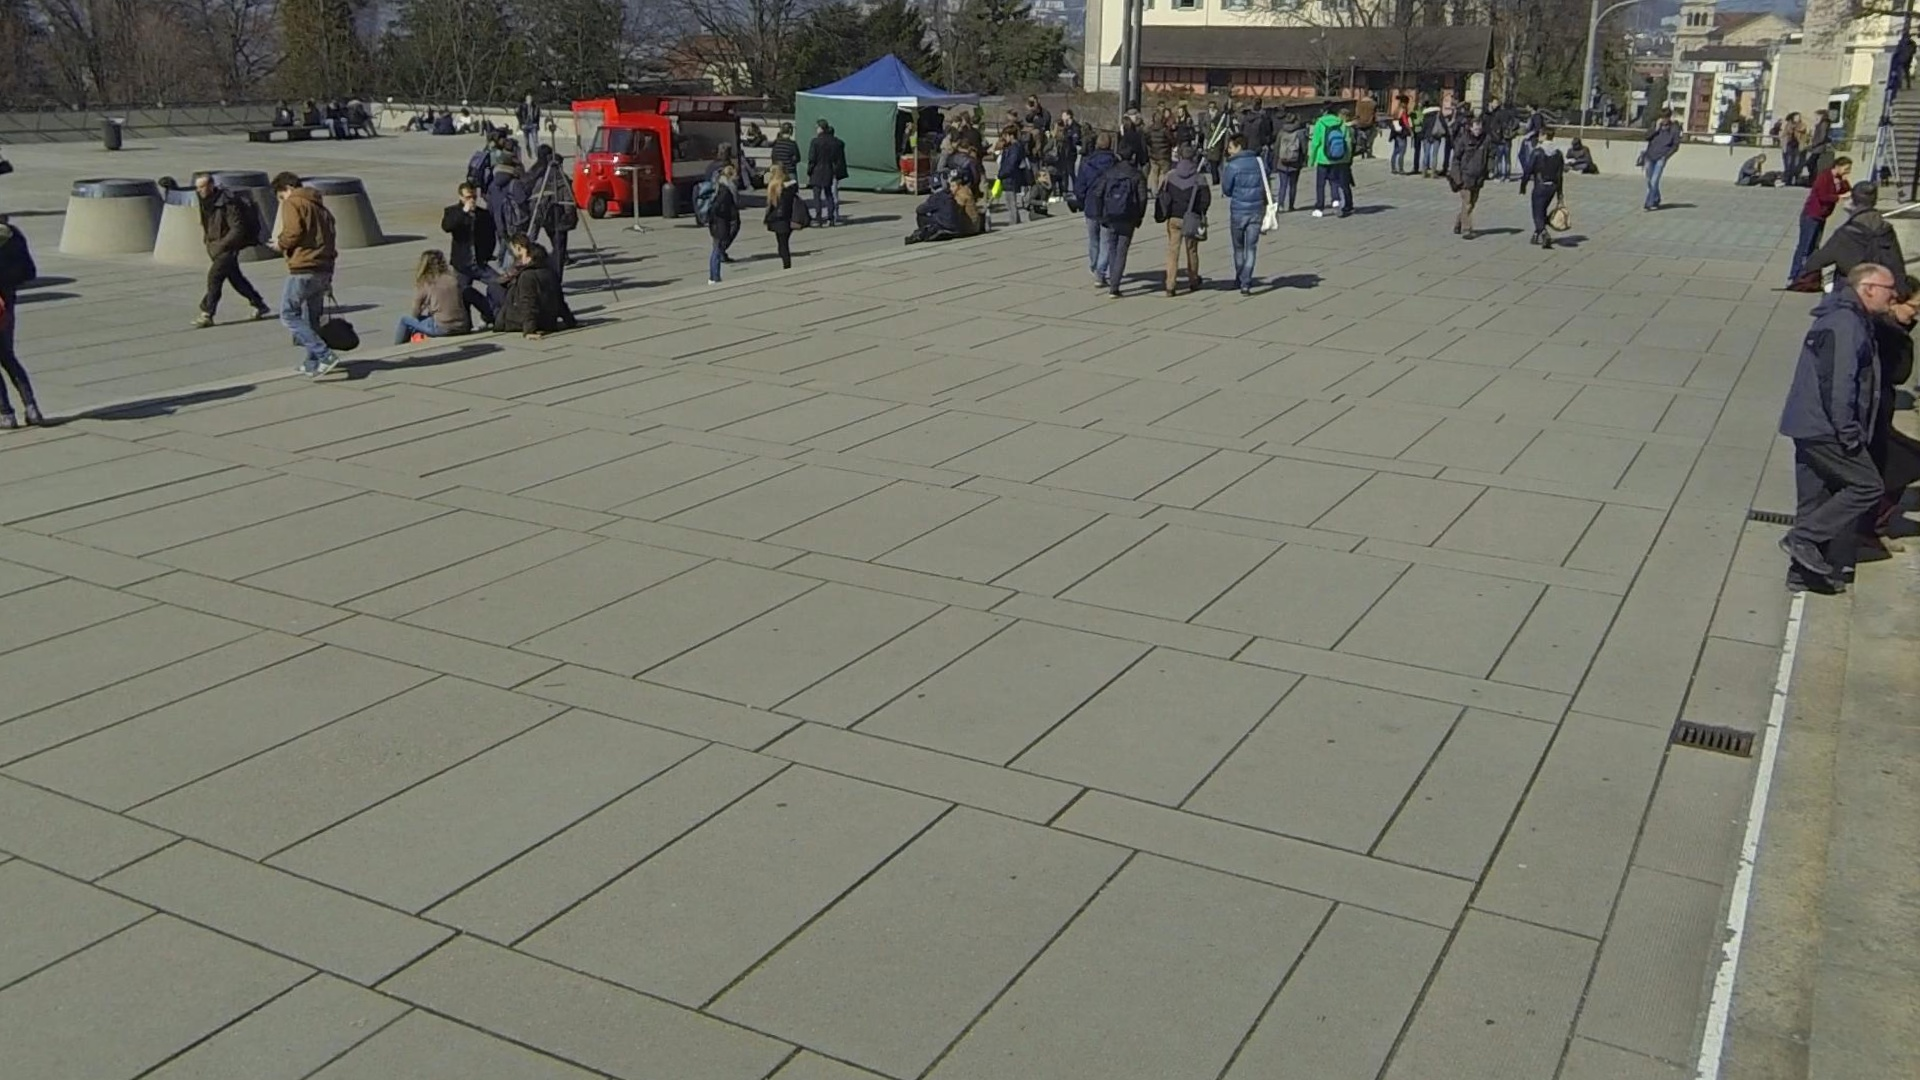
\includegraphics[width=0.4\linewidth]{after_undistort.jpg}}
  \caption{去畸变处理示例}
  \label{undistortion}
\end{figure}

针孔摄像机会引起图像的严重畸变,主要有径向畸变和切向畸变。径向畸变使直线看起来是曲线。离图像中心越远,图像的径向畸变越大。径向畸变可以表示为:
$$
\begin{aligned}
x_{\text{distorted}} = & x(1+k_{1}r^{2}+k_{2}r^{4}+k_{3}r^{6}) \\\
y_{\text{distorted}} = & y(1+k_{1}r^{2}+k_{2}r^{4}+k_{3}r^{6})
\end{aligned}
$$
同样,切向畸变是由于摄像镜片与成像平面不完全平行造成的。因此,图像中的某些区域可能看起来比预期的更近。切向畸变量可表示为:
$$
\begin{aligned}
x_{\text{distorted}} = & x+[2p_{1}xy+p_{2}(r^{2}+2x^{2})] \\\
y_{\text{distorted}} = & y+[p_{1}(r^{2}+2y^{2})+2p_{2}xy]
\end{aligned}
$$
故需要得到五个畸变参数:
$$
\text{distortion coefficients} = (k_{1}, k_{2}, p_{1}, p_{2}, k_{3})
$$
这些畸变参数一般需要标定求得。但在本文中,由于WildTrack数据集提供了每个相机的畸变参数,因此我们可以直接使用,无需标定。
除此之外,还需要相机内外参数。其中,内部参数是特定于照相机的,包括像焦距$(f_{x},f_{y})$和光学中心$(c_{x},c_{y})$等信息,从而可以创建相机的内参数矩阵(Camera Intrinsics)K,以消除由于特定相机的镜头畸变。相机矩阵是特定于相机的,因此得到后可以在同一相机拍摄的其他图像上重复使用。相机矩阵可表示如下:
$$
K=
\left[
\begin{matrix}
f_{x} & 0 & c_{x} \\\
0 & f_{y} & c_{y} \\\
0 & 0  & 1
\end{matrix}
\right]
$$
而外部参数对应于旋转和平移矢量。实际上,WildTrack数据集也已经提供了每个摄像机的相机内外参数。利用这些参数,我们可以通过经典的去畸变算法,实现对视频提取帧的去畸变操作。由于相机参数未变,所以去畸变处理后视频帧中背景状况与官方提供的图片集背景状况完全一致。至此,完成了数据的扩充和预处理操作。

\section{行人检测算法}

本文中的行人检测算法主要依赖于现成的不需要针对特定场景进行训练的单目行人检测器。从单目检测器得到的行人姿态节点中,我们可以计算出每个行人的足点(即双脚之间所站立的位置点)。后续便可以使用此足点进行数据融合,从而得到三维平面上的位置估计结果。

单目检测器实际上有很多算法,如引言中提到的基于运动检测的经典算法如高斯混合模型分离算法、VIBE算法和CodeBook算法等,但这些传统算法很容易受到环境和背景噪声的影响,而且不能检测静止目标,在机器学习方法迅速发展的今天已逐渐过时。因此,本文主要在机器学习算法尤其是深度学习方法中进行选取。在主要使用深度学习方法的算法中,一些单目检测器可以同时提供人物的检测框和姿态节点\cite{li2019crowdpose}。这些方法对全身姿态节点的使用可以更有效地处理遮挡问题,因此,我们选用了目前综合性能最好的AlphaPose。在AlphaPose提供的多种模型中,本文选取了以ResNet152为骨干(Backbone),以YOLOv3为探测器,基于MSCOCO数据集\cite{lin2014microsoft}进行训练得到的Fast Pose(DUC)\cite{fang2017rmpe, li2018crowdpose, xiu2018poseflow}模型。这个模型将输入摄像头拍摄的尺寸为 $256 \times 192$ 的图片,输出每张图片中每个人的姿态节点。其中,人物姿态节点的表示方式与MSCOCO数据集\cite{lin2014microsoft}中姿态表示相同,即包含17个姿态节点。在这些节点中,本文只使用了两个脚踝的节点,具体而言,保留了高于阈值 $t_s$ 的脚踝节点。但由于脚踝节点高于地面,并不能代表人的位置,故可以利用两个脚踝节点计算得到一个抵消项$\delta$,如下所示:
\begin{equation*}
 \delta = bb_{y_{max}} - max(la_y, ra_y)
\end{equation*}
其中,$bb_{y_{max}}$为当前行人的检测框下沿的纵坐标,而$la_y$和$ra_y$则分别是行人的左脚踝节点和右脚踝节点。因此,如图~\ref{GroundPoint_Compute}所示,其中红色点为行人姿态节点,蓝色点为行人脚踝节点(Ankle),黄色点为脚踝中点(Midpoint),绿色点为足点(GroundPoint),可见,通过中点向下偏移$\delta$便可以计算得到行人的足点。
\begin{figure}
    \centering
    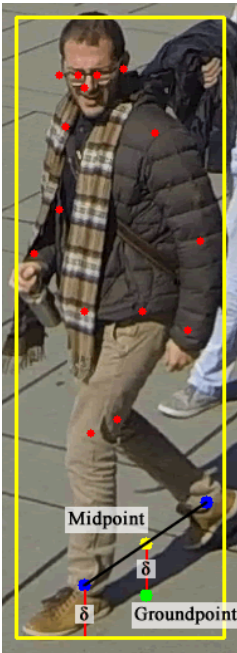
\includegraphics[width=0.2\linewidth]{GroundPoint_Compute.png}
    \caption{行人足点计算实例}
    \label{GroundPoint_Compute}
\end{figure}
根据上述方法,便可输入所有需要的图片或视频数据,推断出每帧中每个行人在此帧上的足点位置坐标,作为后续三维位置推断的基础。

\section{相机投影原理}

在行人检测中,得到每帧每个行人在当前帧的足点位置坐标后,接下来需要推断得到行人在实际地面上的坐标。这里主要使用几何约束和相机投影关系来实现。

相机成像的过程可表示为
$$ \bm{p} = K\bm{P}_{c} $$
其中,$\bm{p}=(\mu, \nu)$是图像中像点的像素坐标,$K$为上文提到的相机内参数矩阵,$\bm{P}_{c}=(X_{c}, Y_{c}, Z_{c})$是相机坐标系下的三维点坐标。然而,相机坐标系并非“稳定”坐标系,因为这个坐标系会随着相机的移动而改变坐标的原点和各个坐标轴的方向。于是引进了稳定不变的世界坐标系。在世界坐标系中,设$\bm{P}_{w}$是在世界坐标系下的坐标,有
$$ \bm{P}_{c} = R\bm{P}_{w} + \bm{t} $$
其中,$R$为$3 \times 3$旋转矩阵,$\bm{t}$为$3 \times 1$为平移向量。将上述公式写为齐次坐标的方式,如下所示:
\begin{equation*}
  \left[
    \begin{array}{c}X_c\\Y_c\\Z_c\\1\end{array}
  \right] 
  = 
  \left[
    \begin{matrix}
      R_{11} & R_{12} & R_{13} & t_1 \\\
      R_{21} & R_{22} & R_{23} & t_2 \\\
      R_{31} & R_{32} & R_{33} & t_3 \\\
      0 & 0 & 0 & 1
    \end{matrix}
  \right]
  \left[
    \begin{array}{c}X_w\\Y_w\\Z_w\\1\end{array}
  \right]
\end{equation*}
即
\begin{equation*}
\left[
  \begin{array}{c}X_c\\Y_c\\Z_c\\1\end{array}
\right] = 
\left[
  \begin{matrix}R&t\\0^\top&1\end{matrix}
\right]
\left[
  \begin{array}{c}X_w\\Y_w\\Z_w\\1\end{array}
\right]
\end{equation*}
于是推导得到相机的外参数(Camera Extrinsics)
\begin{equation*}
T = \left[\begin{matrix}R&t\\0^\top&1\end{matrix}\right]
\end{equation*}
将上式代入$ P_{c} = RP_{w} + t $可得

\begin{equation*}
  \left[\begin{array}{c}\mu\\\nu\\1\end{array}\right]
   = 
  \left[
    \begin{matrix}
      f_x & 0 & c_x & 0 \\\
      0 & f_y & c_y & 0 \\\
      0 & 0 & 1 & 0
    \end{matrix}
  \right]
  \left[
    \begin{array}{cc}R&t\\0^\top&1\end{array}
  \right]
  \left[
    \begin{array}{c}X_W\\Y_W\\Z_W\\1\end{array}
  \right]
\end{equation*}

即得到了将真实场景中的三维点投影到二维的成像平面的相机投影关系。
在上述关系中,我们可以令世界坐标系中的$Z_{w}=0$,从而得到从图像平面到实际地面的单应性矩阵(Homography Matrix)。记相机外参数为$T = [R|\bm{t}]$,则图像平面上一点$\bm{m}=(x,t)^\top$到地面上一点$\bm{M}=(X,Y,0)^\top$的映射关系由下式给出:
\begin{equation*}
  \begin{aligned}
    s\left(
      \begin{matrix}
        \mu \\ \nu \\ 1
      \end{matrix}
    \right)
    &=K\left[
      \begin{matrix}
        \bm{R}^{1}&\bm{R}^{2}&\bm{R}^{3}&\bm{t}
      \end{matrix}
    \right]
    \left(
      \begin{matrix}
        X \\ Y \\ 0 \\ 1
      \end{matrix}
    \right) \\
    &=K\left[
      \begin{matrix}
        \bm{R}^{1}&\bm{R}^{2}&\bm{t}
      \end{matrix}
    \right]
    \left(
      \begin{matrix}
        X \\ Y \\ 1
      \end{matrix}
    \right) \\
    &=H^{-1}
    \left(
      \begin{matrix}
        X \\ Y \\ 1
      \end{matrix}
    \right)
  \end{aligned}
\end{equation*}
其中,$s$为归一化参数,$\bm{R}^{i}$是$R$的列向量,$H$为得到的单应性矩阵。依据上式,就可以将所得行人在图片上的足点投影到实际地面,得到在地面上的足点坐标。同时,需要舍弃那些投影在关注区域外的行人足点。
另一方面,由于后续二维高斯概率分布建模的需要,此处还需要得出上文得到的每个行人地面足点所来源相机的视角方向。为了达到这一目标,我们可以令世界坐标系中的$Z_{w}=1$,则与上文方法相同,可以得到
\begin{equation*}
  \begin{aligned}
    s\left(
      \begin{matrix}
        \mu \\ \nu \\ 1
      \end{matrix}
    \right)
    &=K\left[
      \begin{matrix}
        \bm{R}^{1}&\bm{R}^{2}&\bm{R}^{3}&\bm{t}
      \end{matrix}
    \right]
    \left(
      \begin{matrix}
        X \\ Y \\ 1 \\ 1
      \end{matrix}
    \right) \\
    &=\left[
      \begin{matrix}
        \bm{R}^{1}&\bm{R}^{2}&\bm{R}^{3}+\bm{t}
      \end{matrix}
    \right]^{-1}K^{-1}
  \end{aligned}
\end{equation*}
于是,根据人物在图片上的足点可得到从摄像头到实际地面足点之间射线上的另一点,即射线上$Z_{w}=1$的点。因此,容易得到此行人从来源相机到其地面足点射线的单位方向向量$\bm{v}$。根据上文得到的行人足点和此方向向量便可以进行下一步中二维高斯概率分布的建模。

\section{高斯概率分布建模}

现在已经得到每个行人来源于每个相机在地面上的足点估计坐标。但很明显,上述方法比较比较简单,得到的位置估计准确性难以满足要求。另外,由于WildTrack数据集共有七个摄像头,因此每个行人在地面上的足点估计有七个,所以需要对地面上的足点进行融合,即把同一个人来自七个摄像头的足点坐标融合为一个坐标。在下一章中,我们将进行融合操作。由于当前人物在地面的位置估计并不准确,而其准确性主要与摄像机的距离和摄像机视角有关。可以想到,距离摄像机更近的足点置信水平更高,更远的点则置信水平会比较低。另一方面,由于单个摄像头视角固定,对一个行人左右水平位置的置信水平更高,而对其摄像头视角纵深方向位置的置信水平会比较低。综合来看,单个行人单个摄像头的足点估计可以由一个二维高斯概率分布(Two-dimensional Gaussian distribution)来估计,此二维高斯概率分布的形状大致呈长轴方向为摄像头视角纵深方向、短轴方向为摄像头横向的椭圆形。

二维高斯概率分布的密度函数为:
\begin{equation*}
  \begin{aligned}
    f(x,y)=\frac{1}{2\pi\sigma_{1}\sigma_{2}\sqrt{1-\rho^{2}}}
    e^{
      -\frac{1}{2(1-\rho^{2})}\left(
        \frac{(x-\mu_{1})^{2}}{\sigma_{1}^{2}} - \frac{2\rho(x-\mu_{1})(y-\mu_{2})}{\sigma_{1}\sigma_{2}} 
        + \frac{(y-\mu_{2})^{2}}{\sigma_{2}^{2}}
        \right)
      }
  \end{aligned}
\end{equation*}
其中$\mu_{1},\mu{2},\sigma{1},\sigma{2},\rho$都是常数,可记作:
\begin{equation*}
  \bm{\mu}=\left(
    \begin{matrix}
      \mu_{1} \\ \mu_{2}
    \end{matrix}
  \right),
  \Sigma=\left(
    \begin{matrix}
      \sigma_{1}^{2} & \rho\sigma_{1}\sigma_{2} \\
      \rho\sigma_{1}\sigma_{2} & \sigma_{2}^{2}
    \end{matrix}
  \right)
\end{equation*}
可通过上述两个参数确定此二维高斯概率分布。对于当前来源于特定相机的特定行人足点进行建模,根据相机投影关系,容易得到高斯概率中心点$\bm{\mu}$即为其地面足点坐标。由于当前行人足点从来源相机到其地面足点射线的单位方向向量为$\bm{v}$,记其垂直方向的单位方向向量为$\bm{v}'$,可令
\begin{equation*}
C=k_{c}\bm{v}^\top\bm{v}, C'=k_{c}\bm{v}'^\top\bm{v}'
\end{equation*}
则二维高斯概率分布中
\begin{equation*}
  \left\{
    \begin{aligned}
      \mu & = (X_{w}, Y_{w})^\top \\
      \Sigma & = kC + (1-k)C'
    \end{aligned}
  \right.
\end{equation*}
其中$k$为高斯概率形状调整参数,若$k\rightarrow1$,则二维高斯概率趋于扁平,长轴方向为$\bm{v}$,若$k\rightarrow0$,则二维高斯概率趋于扁平,长轴方向为$\bm{v}'$,若$k\rightarrow0.5$,则二维高斯概率趋于一个圆形。
从而,根据上述方法可以建立单个行人单个摄像头的足点估计的二维高斯概率分布,对于单个摄像头的建模结果如图~\ref{a}所示,其中黄色三角为真实标注点,不同颜色的分布为高斯概率分布。
% \begin{figure}
%   \centering
%   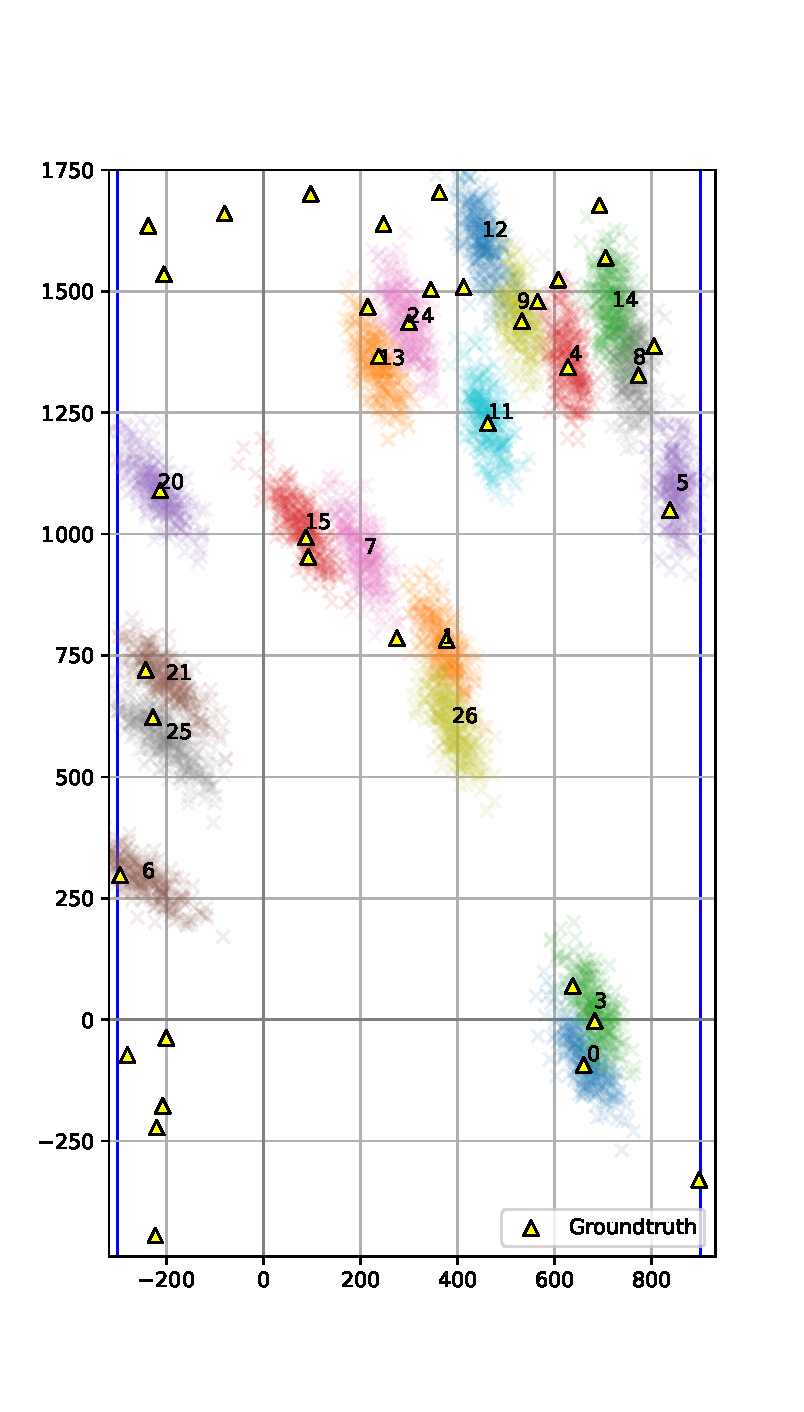
\includegraphics[width=0.4\linewidth]{oneCam_gaussian.png}
%   \caption{单个摄像头二维高斯概率分布建模}
%   \label{oneCam_gaussian}
% \end{figure}
对于WildTrack数据集,将七个摄像头所得行人在地面上的足点进行二维高斯概率分布建模后,投影在同一张图上,如图~\ref{b}所示,其中黄色三角为真实标注点,相同颜色的椭圆为同一摄像头来源的二维高斯概率分布建模。
% \begin{figure}
%   \centering
%   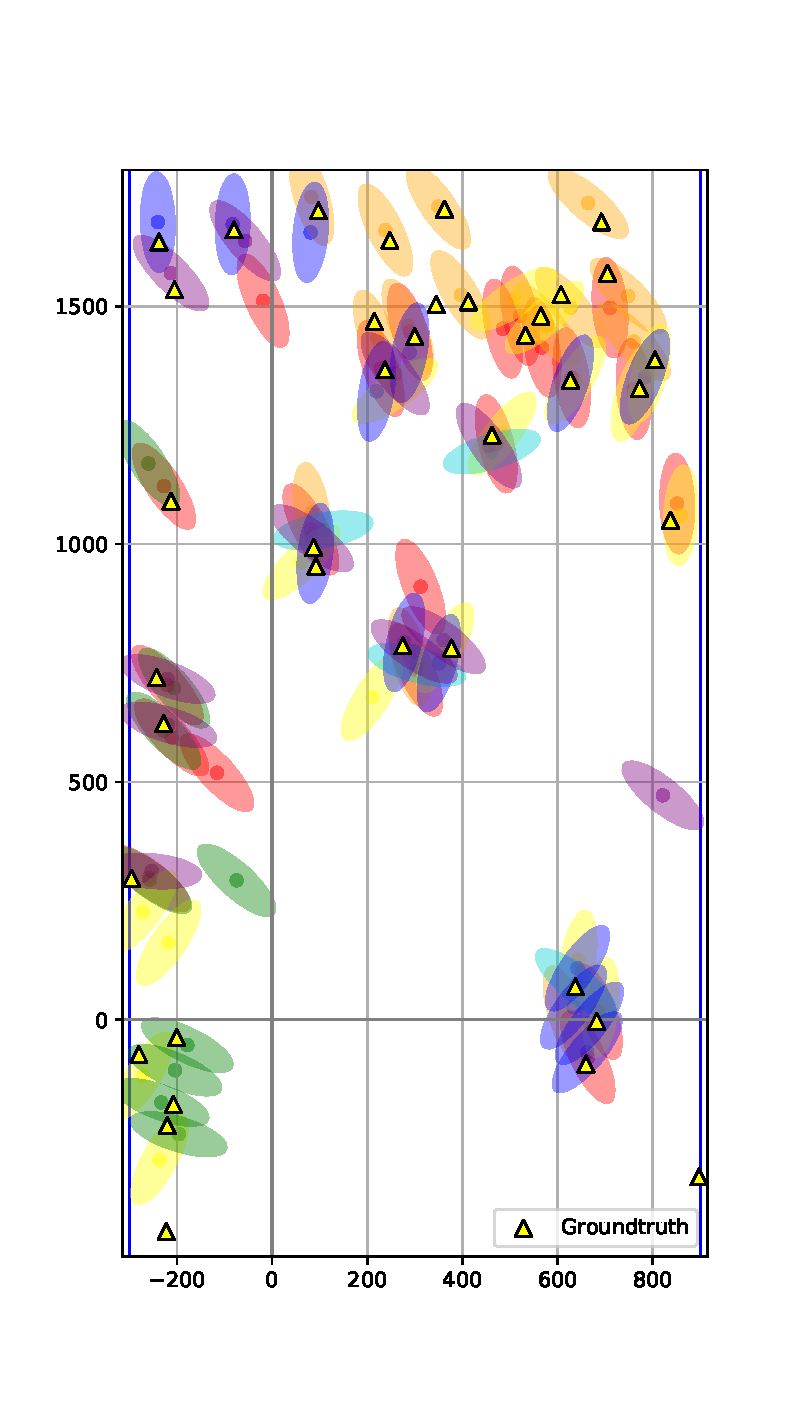
\includegraphics[width=0.35\linewidth]{multi-cam_gaussian.pdf}
%   \caption{单个摄像头二维高斯概率分布建模}
%   \label{multiCam_gaussian}
% \end{figure}
\begin{figure}
  \centering
  \subcaptionbox{\label{a}}
    {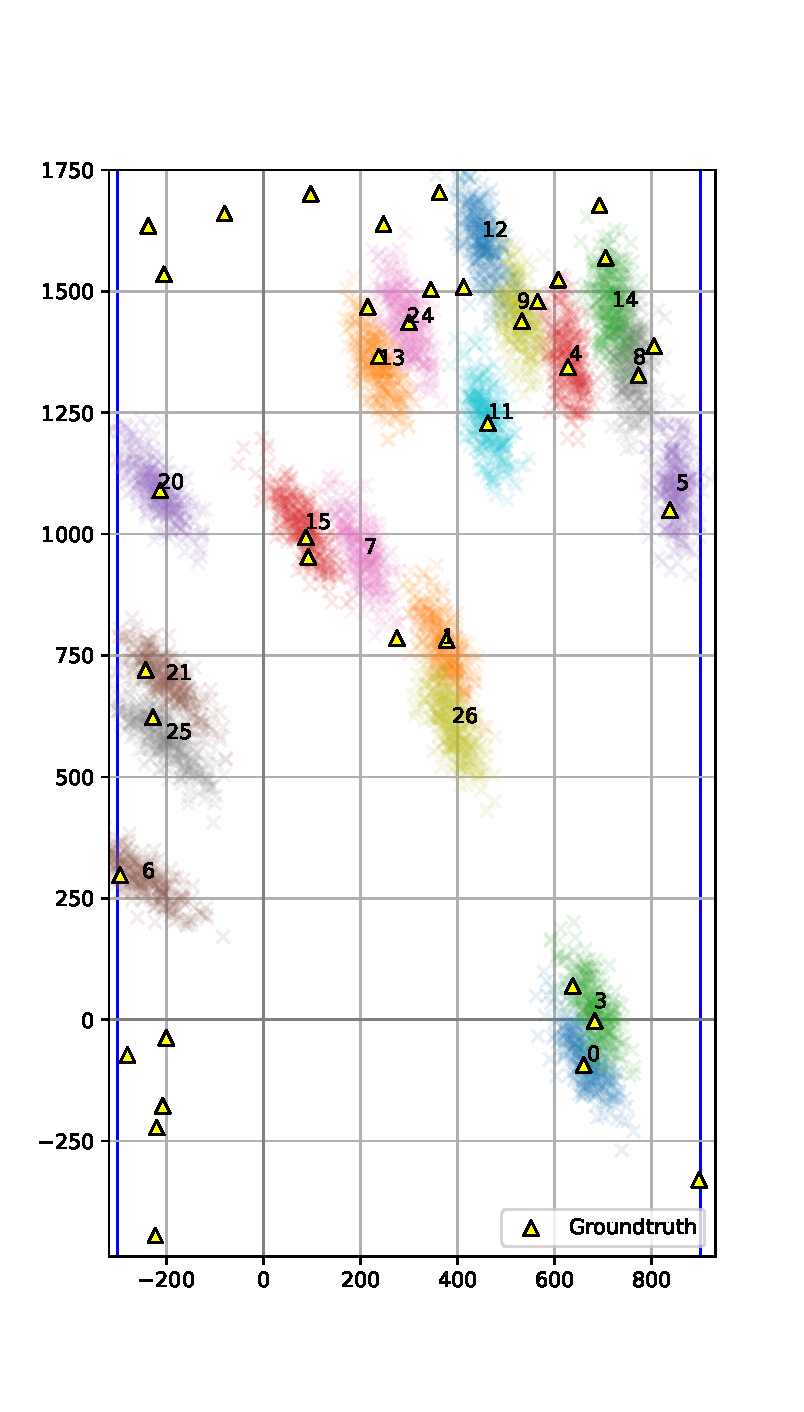
\includegraphics[width=0.4\linewidth]{oneCam_gaussian.pdf}}
  \subcaptionbox{\label{b}}
    {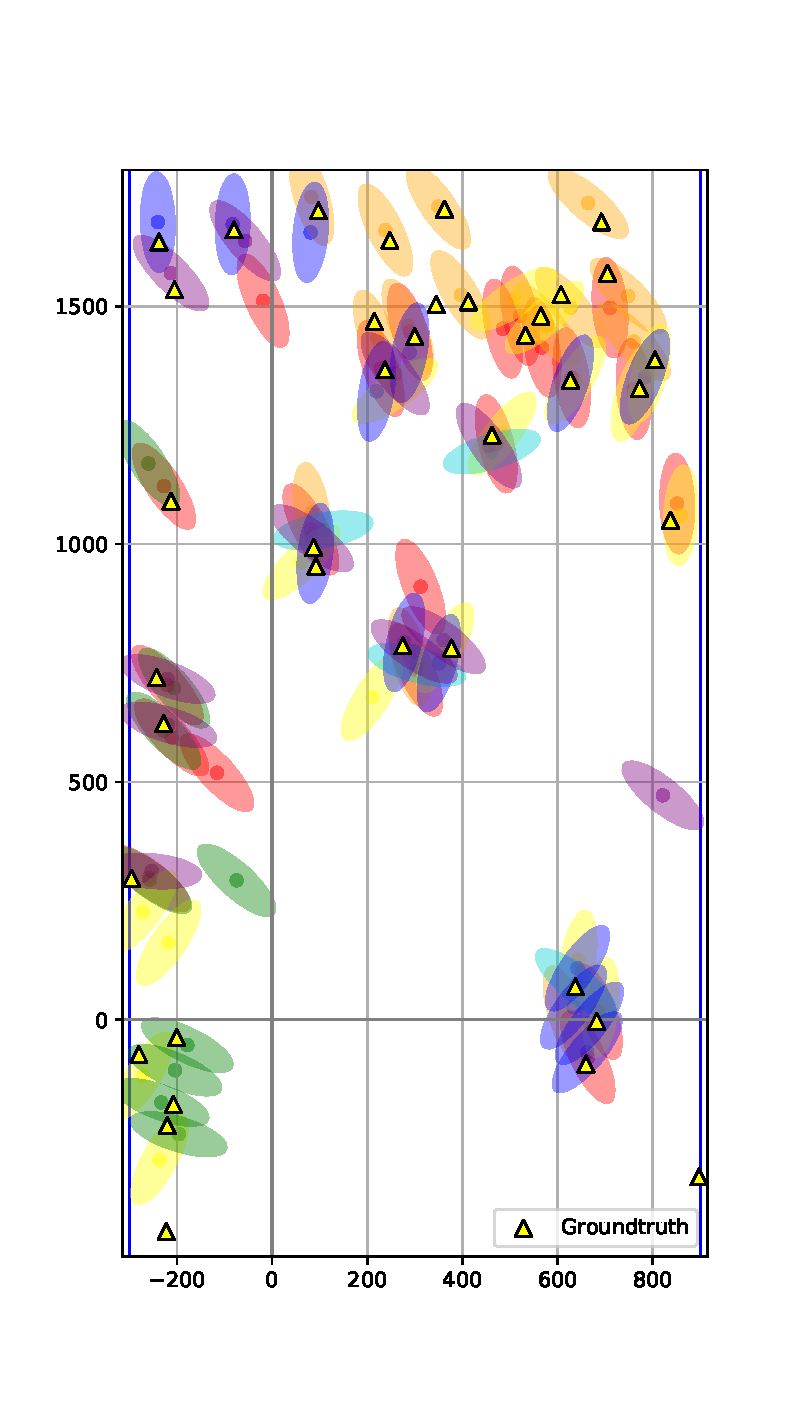
\includegraphics[width=0.4\linewidth]{multi-cam_gaussian.pdf}}
  \caption{多个分图的示例}
  \label{gaussian}
\end{figure}


\section{本章小结}

本章主要内容为深度学习算法的前置步骤。首先介绍了数据集的扩充和预处理过程,然后说明了所使用的现成行人检测算法的选取和具体实现细节,之后比较详细地介绍了相机投影原理和如何利用相机投影对得到的行人姿态节点进行处理,从而计算出行人的实际地面位置坐标,最后,详细介绍了所采用的二维高斯概率分布建模原理,阐明了所得行人地面位置坐标和相机参数如何决定了高斯概率分布的参数。这些步骤,为后续的数据融合和深度学习算法的使用做了铺垫。